\chapter{Konzept}
\section{Allgemeines}
\subsection{Zweck}

\subsection{Ausgangslage}
Der Abschnitt hier basiert auf dem vorangehenden Entscheid bei der Auswahl des Rich Client Frameworks. Aus den im Abschnitt \titleref{rcp_entscheid} beschriebenen Gründen wird zur Implementation des Garbage Collection Log Analyzers die Eclipse Rich Client Plattform in der Version 3.x\footnote{die aktuelle Version ist 3.7 (stand: 31.8.2011)} genommen. Die in der Anforderungsanalyse allgemein definierten Anforderungen werden nun spezifisch auf diese Plattform konzipiert, für die einzelnen Thematiken werden nun auch die Begrifflichkeiten innerhalb Eclipse verwendet.


\section{Umgebung}
\subsection{Lizenzierung}
Die Software wird lizenziert unter der Eclipse Public License\footnote{http://www.eclipse.org/legal/epl-v10.html} in der Version 1.0. Dies ist eine freie Software-Lizenz und gewährt das Recht zur freien Nutzung, Weiterverbreitung und Veränderung der Software. Die Benutzung einer Open-Source Lizenz hat insbesondere folgende Vorteile:
\begin{itemize}
	\item An der Entwicklung von Open-Source Software können sich eine beliebige Anzahl an Entwicklern beteiligen. Der Entwicklungsaufwand kann skaliert werden.
	\item Jedermann kann Erweiterungen entwickeln oder Fehler beheben.
\end{itemize}

Bei der Wahl der Lizenz muss gleichzeitig in Betracht gezogen werden, dass die Lizenzen der verwendeten Bibliotheken ebenfalls eingehalten werden. Übersicht der verwendeten Bibliotheken:



\begin{longtable}{|p{3cm}|p{7cm}|p{4cm}|}
    \caption{Verwendete Bibliotheken und deren Lizenzen}\\\hline
	\textbf{Bibliothek} & \textbf{Beschreibung}  & \textbf{Lizenz}\\\hline
	Eclipse Framework & Framework zur Erstellung von Destkop-Anwendungen. & Eclipse Public License\\\hline 
	JFreeChart & Wird für im Bereich des Reportings verwendet um Graphiken und Charts anzuzeigen. & Lesser General Public License\footnote{http://www.gnu.org/licenses/lgpl.html}\\\hline
\end{longtable}

\subsection{Build-Automation}
Die Automatisierung des Software-Builds ist hinsichtlich der Integration in ein Continuous Integration System Voraussetzung. Es hat zusätzlich aber andere Vorteile:
\begin{itemize}
	\item Tasks wie das Kompilieren, die Packetierung und das Deployment der Software müssen nicht mehr manuell gemacht werden.
	\item Zur Verhinderung von Regression und entsprechend zur Gewährleistung der Qualität können vor jedem Release automatisch die Tests durchgeführt werden.
\end{itemize}


Als Werkzeug zum automatisierten Build der Software wird Maven Tycho\footnote{Im Bereich der Eclipse Rich Client Entwicklung kann entweder PDE Build, ein auf Apache Ant basiertes Build-System für Eclipse RCP Applikationen\cite{vogelZapfPdeBuild} oder die Maven-Integration Tycho (http://tycho.sonatype.org) verwendet werden.} verwendet. Um Tycho führt mittlerweile kein Weg drum herum, es hat im Vergleich zum PDE Build einige Vorteile:
\begin{itemize}
	\item Maven Builds lassen sich ohne grossen Aufwand in Continuous Integration Systeme integrieren.
	\item Maven hat eine gute Integration in alle gängigen Entwicklungsumgebungen\footnote{Projekt-Dateien müssen nicht mehr in die Versionskontrolle eingecheckt werden.} und ist sehr verbreitet
\end{itemize}

\subsection{Continous Integration}
Als Continuous Integration Server wird Jenkins\footnote{http://jenkins-ci.org - Jenkins ist der ehemalige Hudson CI Server, welcher nach dem Kauf von Sun durch Oracle als Branch entstanden ist.} verwendet. Jenkins bringt nebst seiner Benutzerfreundlichkeit als Build Server einige zum Projekt nötigen Voraussetzungen mit:
\begin{itemize}
	\item Jenkins ist für alle denkbaren Betriebssysteme vorhanden.
	\item Jenkins ist kompatibel mit allen gängigen Systemen zur Versionskontrolle: Git, Subversion, CVS, etc.
	\item Maven-Projekte lassen sich ohne grossen Aufwand als Build-Projekte konfigurieren.
\end{itemize}

\subsection{Versionskontrolle}
Zur Versionskontrolle kommen mehrere Werkzeuge in Frage. Git\footnote{http://git-scm.com} ist ein verteiltes Sourcecode Management System und ist konzeptionell und hinsichtlich Benutzerfreundlichkeit besser als Subversion und CVS\footnote{Git kann offline verwendet werden, das Verschieben von Verzeichnissen führt nicht zu Problemen, etc.}. Auf der Plattform Github\footnote{http://github.com} kann man öffentliche Projekte gratis ``hosten''.

\subsection{Issue Tracker}
Als Issue Tracker wird Jira verwendet. Es handelt sich dabei um eine kostenpflichtige aber relativ günstige Software für das Issue-Tracking.

\subsection{Installation der Software}\label{installation}
Zur Installation der Software benötigt man die Eclipse-Entwicklungsumgebung in der Version 3.7. Darin integriert befindet sich ein Update-Manager, der Software-Komponenten von Lokal oder dem Netzwerk installieren kann. Auch Updates werden über diesen Mechanismus installiert. Die Analyse-Software wird via eine Update-Seite bereitgestellt. Der Software-Build durch das Continuous Integration System publiziert die Artefakte (Features, Plugins) auf einen via Internet zugänglichen Rechner, von welchem der Update-Manager die Software herunterlädt um anschliessend zu importieren. Update-Seiten im Eclipse-Umfeld bestehen aus Features (Eclipse Feature-Projekt). Features bestehen aus unterschiedlichen Plugins (Eclipse Plugin-Projekt). Eclipse\footnote{in der Basis ist es Equinox, die Implementation des OSGi Standards} ist in der Lage, Plugins zur Laufzeit zu installieren, starten, deinstallieren.

Die Update-Seite für diese Software wird folgendermassen aufgebaut:
\begin{itemize}
	\item Garbage Collection Log Analysis (Kategorie)
		\begin{itemize}
			\item Core (Feature)
			\item JRockit Extension (Feature)
		\end{itemize}
\end{itemize}
Nachträglich kann somit auch für ein anderes Log-Format eine Extension geschrieben werden.


\section{Übersicht}
\subsection{Architektur}
Wie im Abschnitt \titleref{installation} erläutert, besteht die Software aus zwei getrennten Features. Das Core-Feature ist die Basis und verantwortlich für den gesamten Import-Prozess (Import-Wizard, Leseprozess der Log-Datei, Anzeige der Menus, Profil-Verwaltung, etc.). Die JRockit Extension ist eine für die Garbage Collection Logs der JRockit geschriebene Erweiterung. Sie ist für das Parsing der Log-Dateien, die Aufbereitung der Daten und die Anzeige der Charts zuständig. Beinhaltet aber keine Core-Funktionalität.
 \begin{figure}[H]
  	\centering
        	\caption{Architektur: Komponentendiagramm}
    	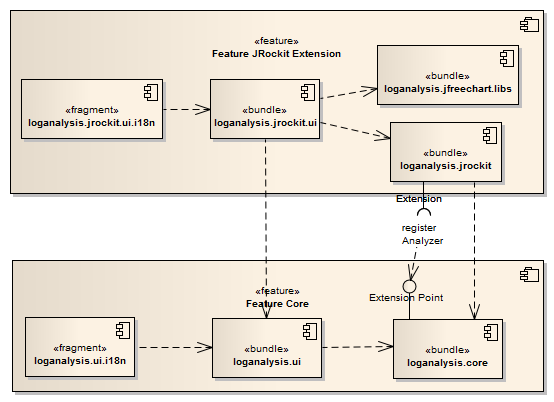
\includegraphics[width=15cm]{images/architektur_komponenten_uebersicht}
\end{figure}

Das Core Feature besteht aus dem Modul User Interface (``loganalysis.core.ui'') und einem von JFace und SWT\footnote{JFace und SWT wird in Eclipse als Library für den Presentation Layer verwendet} unabhängigen Teil (``loganalysis.core''). Öffnet der Benutzer eine Garbage Collection Log Datei, wird diese durch das Core Feature eingelesen und an alle verfügbaren Extensions weitergeleitet. Die erste Extension welche den Inhalt der Datei versteht, öffnet seine dafür vorgesehenen Reports und Charts. Jede Extension hat ein basierend auf dem Log-Format eigenes Domänen-Modell.

\subsection{Weitere Projekte}
Einige Plugins wurden im vorherigen Abschnitt nicht erwähnt:
\begin{itemize}
	\item Features\footnote{Feature-Projekte definieren im Eclipse-Umfeld ein in sich lauffähiges Software-Packet. Via einen Xml-Deskriptor werden die abhängigen Plugin-Projekte definiert und in das Feature gepackt.}
		\begin{itemize}
			\item loganalysis.feature
			\item loganalysis.jrockit.feature
		\end{itemize}
	\item Thirdparty Bibliotheken\footnote{Thirdparty Bibliotheken werden ebenfalls in ein Plugin gepackt, da innerhalb der Eclipse-Runntime nur Plugins installiert werden können. Die ``Plugin-Hülle'' definiert die exportierten und importierten Packete und die Abhängigkeiten.}
		\begin{itemize}
			\item  loganalysis.jfreechart.libs (JFreeChart Library)
		\end{itemize}
	\item Targetplattform\footnote{Die Targetplattform ist eine Konfiguration welche definiert, gegen welche Plattform die Anwendung entwickelt wird.}
		\begin{itemize}
			\item  loganalysis.targetplatform (beinhaltet die Target-Plattform)
		\end{itemize}
	\item Update-Seite\footnote{Die Konfiguration innerhalb eines Projekts zur Erstellung einer Update-Seite definiert die auf der Seite publizierten Features.}
		\begin{itemize}
			\item loganalysis.updatesite (definiert und generiert die Update-Seite)
		\end{itemize}
\end{itemize}

\section{Basissoftware (Core)}
\subsection{Ablauf Garbage Collection Analyse}
Nach dem Import der sich auf einem lokalen Laufwerk befindenden Log Datei befindet sich diese im Fenster ``Log Files''. Beim Doppelklick auf diese Datei wird der Analyse-Vorgang gestartet. Mit der Voraussetzung, dass die JRockit Extension (Feature) installiert ist, passiert danach folgendes:
\begin{enumerate}
	\item Die Garbage Collection Log Datei wird eingelesen und im FileDescriptor gespeichert.
	\item Für alle durch Extensions registrierte Log-File Analyzer, wird abgefragt, ob er die Datei versteht.
	\item Dem ersten dieser Analyzer wird dieses FileDescriptor Objekt übergeben um den Inhalt zu prozessieren. Als Resultat wird ein Objekt vom Typ IJvmRun erwartet. Zusätzlich dazu wird der Identifikator des zu öffnenden Analyse-Fensters zurückgeliefert.
	\item Der passende Analysebildschirm (befindet sich innerhalb der Extension) wird geöffnet.
\end{enumerate}
\subsubsection{Domänenmodell}
 \begin{figure}[H]
  	\centering
        	\caption{Domänenmodell: Garbage Collection}
    	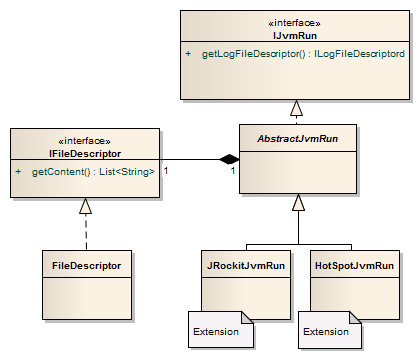
\includegraphics[width=11cm]{images/core_domain}
\end{figure}
\textit{IFileDescriptor} wird für die Abstraktion der Garbage Collection Log Datei verwendet. Darin enthalten sind Metadaten wie Dateiname und Pfad sowie der Inhalt der Datei - dieser wird allerdings erst beim öffnen der Analyse geladen (lazy). Das Basis-Modell beinhaltet zusätzlich eine naive Abstraktion eines Runs: \textit{IJvmRun} und \textit{AbstractJvmRun}. Diese werden dann in der jeweiligen Extension realisiert (Beispiel: \textit{JRockitJvmRun}). 

\subsection{Profilverwaltung}
Die Definition von benutzerdefinierten Analysen kann innerhalb von Profilen gespeichert werden. Diese Profile werden in einer Übersicht dargestellt und sind gruppiert nach der jeweiligen Extension (Beispiel: JRockit). Sofern eine Log-Datei geöffnet oder selektiert ist, kann durch Doppelklick auf ein gespeichertes Profil die Analyse dafür geöffnet werden. Die Implementation der View-Domäne befindet sich in der jeweiligen Extension. Damit das Profil über die View ``Profiles'' ersichtlich ist, muss es \textit{IProfile} realisieren.
\subsubsection{Domänenmodell}
 \begin{figure}[H]
  	\centering
        	\caption{Domänenmodell: Profilverwaltung}
    	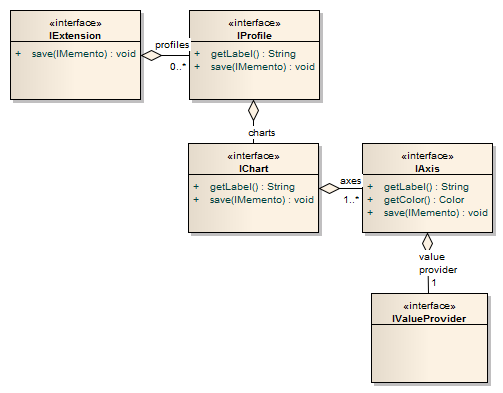
\includegraphics[width=13cm]{images/core_domain_profiles}
\end{figure}
\textit{IExtension} ist eine Abstraktion der Extension und dient zur Gruppierung der für die Extension angelegten Profile. Innerhalb eines Profils können unterschiedliche Diagramme (\textit{IChart}) angelegt werden, welche wiederum durch Achsen (\textit{IAxis}) und deren Daten. Die Abfrage der Daten findet über sogenannte \textit{IValueProvider} statt. Diese definieren den Weg, wie die Daten aus dem Domänen-Modell gelesen werden.

\section{JRockit Erweiterung (JRockit Extension)}
\subsection{Parsen JRockit Garbage Collection Log Datei}
Die Garbage Collection Logs der JRockit Virtual Machine bestehen aus Einträgen unterschiedlicher Log Modulen. Genauer genommen ist es eine Log-Datei, bei welcher die Informationen zur Garbage Collection und Memory Allokation eingeschaltet werden können (siehe Abschnit \ref{logmodule} \titleref{logmodule}). Für die Garbage Collection Analyse sind nur ein Teil dieser Einträge interessant - es werden also niemals alle dieser Einträge von der Analyse-Software verstanden. Für die Analyse der Einträge ist der \textit{JRockitAnalyzer} zuständig.Die Einträge werden durch einen Prozessor, der nach dem Chain-of-Responsibility Pattern\cite{wiki:chainOfResponsibilityPattern} aufgebaut ist, prozessiert. Die wichtigsten Einträge des Garbage Collection Logs sind die des Memory Modules (\textit{MemoryModuleProzessor}). 




 \begin{figure}[H]
  	\centering
        	\caption{JRockit Analyseprozess}
    	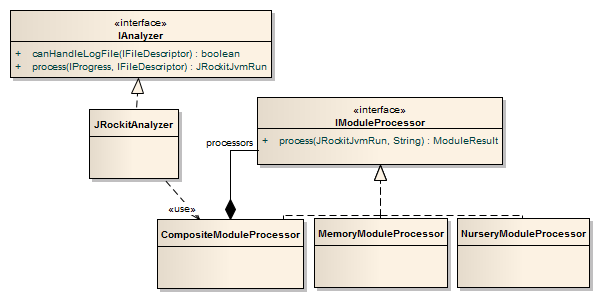
\includegraphics[width=16cm]{images/jrockit_log_processing}
\end{figure}

\subsection{JRockit Garbage Collection}
\begin{landscape}
 \begin{figure}[H]
  	\centering
        	\caption{Domänenmodell: Garbage Collection (JRockit Implementation)}
    	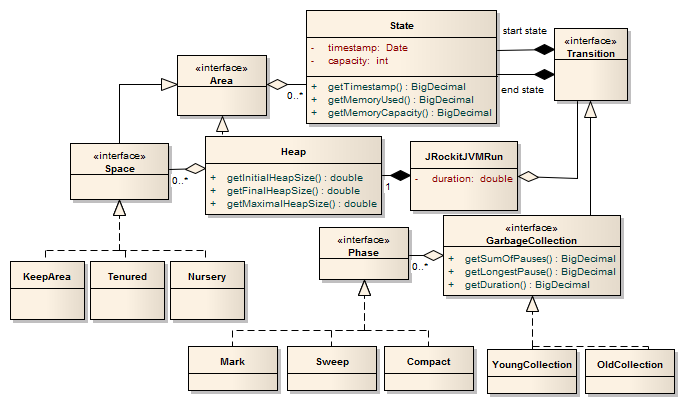
\includegraphics[width=19.5cm]{images/jrockit_extension_domain}
\end{figure}
\end{landscape}
\subsection{Charts, Reports}

\section{Funktionalitäten}
\subsection{Software-Installationsprozess}
\subsubsection{Relevante Requirements}
\begin{itemize}
	\item UC-A-01 (Software installieren)
	\item UC-A-02 (Software updaten)
	\item UC-E-01 (Neuer Software-Release erstellen)
	\item QA-01 Installierbarkeit
\end{itemize}


\subsection{Import JRockit}
\subsubsection{Relevante Requirements}
\begin{itemize}
	\item UC-A-03 (Garbage Collectio nLog Datei importieren)
\end{itemize}

\subsection{Analyse JRockit}
\subsubsection{Relevante Requirements}
\begin{itemize}
	\item UC-A-04 (Garbage Collection Log Datei analysieren)
	\item UC-A-04-a (Statistik Übersicht)
	\item UC-A-04-b (Heap Benutzung)
	\item UC-A-04-c (Dauer Garbage Collection)
	\item UC-A-04-d (Benutzerdefinierte Auswertung)
\end{itemize}




